\documentclass[a4paper]{scrreprt}
\usepackage[german]{babel}
\usepackage[utf8]{inputenc}
\usepackage{graphicx}
\usepackage{pdflscape}

\begin{document}
\title{Implementierungsdokument}
\author{Hanselmann, Hecht, Klein, Schnell, Stapelbroek, Wohnig}
\date{\today\\v0.2}
\maketitle 
\tableofcontents	
\listoffigures


\chapter{Einleitung}
Dieses Dokument beschreibt die Implementierungsphase einer Praxis der Softwareentwicklungsgruppe am Karlsruher Institut für Technologie. Der Titel der Gruppenaufgabe lautet: \textit{Entwicklung eines Werkzeugs zur Analyse formaler Eigenschaften von Wahlverfahren}. \\
Diese Dokument stellt die in dieser Phase entstandenen Unterschiede zu den vorherigen Phasen (Pflichtenheft und Entwurf) dar und erklärt, warum diese notwendig wurden. \\
Weiterhin wird die zeitliche sowie die personelle Aufteilung der Implementierung vorgestellt. \\
\section{Ziel des Programmes}
Ziel des Programmes ist es, eine Lösung zur Analyse von formalen Eigenschaften von Wahlverfahren zu präsentieren. Zur Analyse der Eigenschaften wird Bounded Model Checking (Glossareintrag) verwendet. Der verwendete Bounded Model Checker ist CBMC (Glossareintrag). Das Programm soll folgende Module bereitstellen: 
\begin{itemize}
\item Eine Möglichkeit zur Beschreibung eines Wahlverfahrens in der Programmiersprache C. 
\item Eine Möglichkeit zur Beschreibung von Eigenschaften, auf die das Wahlverfahren geprüft werden soll. Die Beschreibung erfolgt in einer Makrosprache (Glossareintrag).
\item Eine Möglichkeit zum Angeben der Parameter für welche das angegebenen Wahlverfahren analysiert werden soll (Anzahl Wähler, Anzahl Kandidaten, Anzahl Sitze). 
\item Eine Möglichkeit, die Analyse auszuführen.
\item Eine Ausgabe des Ergebnisses der Analyse: Eine Erfolgsmeldung falls alle Eigenschaften erfüllt werden und Präsentation eines Gegenbeispiels sonst.
\end{itemize}


\chapter{Unterschiede zu den im Pflichtenheft gestellten Kriterien}

\section{Kannkriterien}

\subsection{Betrieb auf dem Betriebssytem MacOS} 
Da wir keinen MAC zum Testen hatten, haben wir keine Implementierung für MacOS
vorgenommen. Da unser Entwurf Erweiterungen aber leicht zulässt, ist es für
Benutzer, die dieses Betriebssystem besitzen mit einigen Programmierkenntnisse
möglich sich diese Option selbst einzubauen. Dazu müsste die Funktionalität erstellt werden, Prozesse auf diesem Betriebssystem von Java aus zu starten. Mit dieser müssten dann CMBC sowie GCC angesprochen und deren Ausgabe zurückgegeben werden. Alle anderen Systeme sind unabhängig vom Betriebssystem.

\chapter{Änderungen am Entwurf}
\section{Package Highlevel}

Das Paket \verb!highlevel! bildet den Kern von BEAST. Es enthält die \verb!MainClass!, über die BEAST gestartet wird. Weiterhin enthält es Interfaces zu den anderen Paketen, wodurch diese Pakete unabhängiger von einander sind und damit leichter auszutauschen. Der \verb!CentralObjectProvider! generiert Instanzen dieser Interfaces und stellt sie dem \verb!BEASTCommunicator! bereit. \\

\subsection{CentralObjectProvider}
\verb!AbstractFactory! in \verb!highlevel! ist jetzt keine Abstrakte Fabrik mehr.\\ Dieses Entwurfsmuster konnte nicht verwendet werden, da die zu erstellenden Objekte teilweise voneinander abhängig sind. Weiterhin gibt es Objekte, die mehrere Rollen einnehmen, d.h. sie implementieren unterschiedliche Interfaces (wie etwa der Parametereditor, der sowohl \verb!ParameterSource!, als auch \verb!ProjectSource! und \verb!MainNotifier! implementiert). \\
Deshalb wurde sie durch das Interface \verb!CentralObjectProvider! und die Klasse\\ \verb!PSECentralObjectProvider!, die dieses implementiert, ersetzt. \verb!CentralObjectProvider! verwirklicht die ursprüngliche Funktion der Abstrakten Fabrik, unabhängig von konkreten Implementierungen zu sein. \\
\verb!PSECentralObjectProvider! erzeugt die konkreten Objekte für unsere Implementierung der \verb!highlevel!-Interfaces und stellt diese dem \verb!BEASTCommunicator! zur Verfügung. Dieser muss weiterhin nur von den Interfaces wissen. \\

\subsection{DisplaysStringsToUser}
Es wurde das Interface \verb!DisplaysStringsToUser! hinzugefügt. Es wird von allen Elementen, die dem Nutzer Text anzeigen, implementiert. Damit wird die Einbindung anderer Sprachen vereinfacht. \\

\subsection{start-/stopReacting}
Allen Interfaces zu Paketen mit GUI wurden die Methoden \verb!stopReacting! und \verb!resumeReacting! hinzugefügt. Diese verhindern, dass der Nutzer während einer laufenden Analyse Änderungen an dafür benötigten Daten vornimmt. \\

\subsection{ProjectSource}
Es wurde das Interface \verb!ProjectSource! hinzugefügt. Es wird von \verb!ParameterEditor! implementiert. Damit wird es möglich, das Speichern und Laden von ganzen Projekten in zukünftigen Versionen leichter einem anderen Fenster als dem Parametereditor zu überlassen. \\
\subsection{isCorrect}
Interfaces zu Paketen, die Daten für die Analyse bereitstellen, wurde die Methode \verb!isCorrect! hinzugefügt. Damit kann vor Start einer Analyse überprüft werden, ob die bereitgestellten Daten frei von Fehlern sind, die die Analyse beeinträchtigen würden.


\section{CodeGenerierung}

Die Klasse \verb!CBMCCodeGeneration! ist nicht mehr statisch. \\
Sie wird in der Implementierung von der Klasse \verb!CBMCProcessFactory! instantiiert. \\
So wird für jedes erzeugte C-Tempfile (Glossareintrag) eine neue Instanz erstellt. Das ist sinnvoll, da es genau von den Parametern abhängt. \\
Jede Instanz der Klasse \verb!CBMCCodeGeneration! erstellt eine Instanz der Klasse \\\verb!CBMCCodeGenerationVisitor!. \\
Diese besitzen zwei neue Methoden, die einstellen, ob er zur Codegenerierung einer Vor- oder Nachbedingungen eines Wahlverfahrens verwendet wird.  \\
(Verändertes Klassendiagramm hier)

\section{UserActions}
Alle \verb!UserActions! der vier GUIs haben jetzt nur noch einen Verweis auf den ihnen zugehörigen Controller, und holen sich von diesem mit Gettern die von ihnen gebrauchten Klassen (\verb!FileChooser!, \verb!SaveBeforeChangeHandler!...). Beispielhaft am \verb!BooleanExpEditor! gezeigt:
\newline

(Diagramm folgt)
\newline

\section{SaverLoader}
\verb!PostAndPrePropertiesDescriptionSaverLoader!, \verb!ElectionDescriptionSaverLoader!, \verb!ElectionCheckParameterSaverLoader! und \verb!ProjectSaverLoader! implementieren nun das Interface \verb!SaverLoader! mit den dargestellten Methoden. Dies ermöglicht es der Klasse \verb!FileChooser!, polymorph gegebene DatenTypen abzuspeichern und gegebene Dateien zu laden.
Alle anderen \verb!SaverLoader!-Klassen haben nur statische Methoden.
Zudem gibt es noch eine \verb!StringSaverLoader! Klasse, die mit \verb!createSaveString! aus allen vom Nutzer editierbaren Strings alle Vorkommen von ">" durch ">>" ersetzt, beziehungsweise dies mit !\verb!createFromSaveString! rückgängig macht. Dies verhindert die Erstellung von nicht ladbaren Dateien trotz valider Nutzer-Eingaben.\\
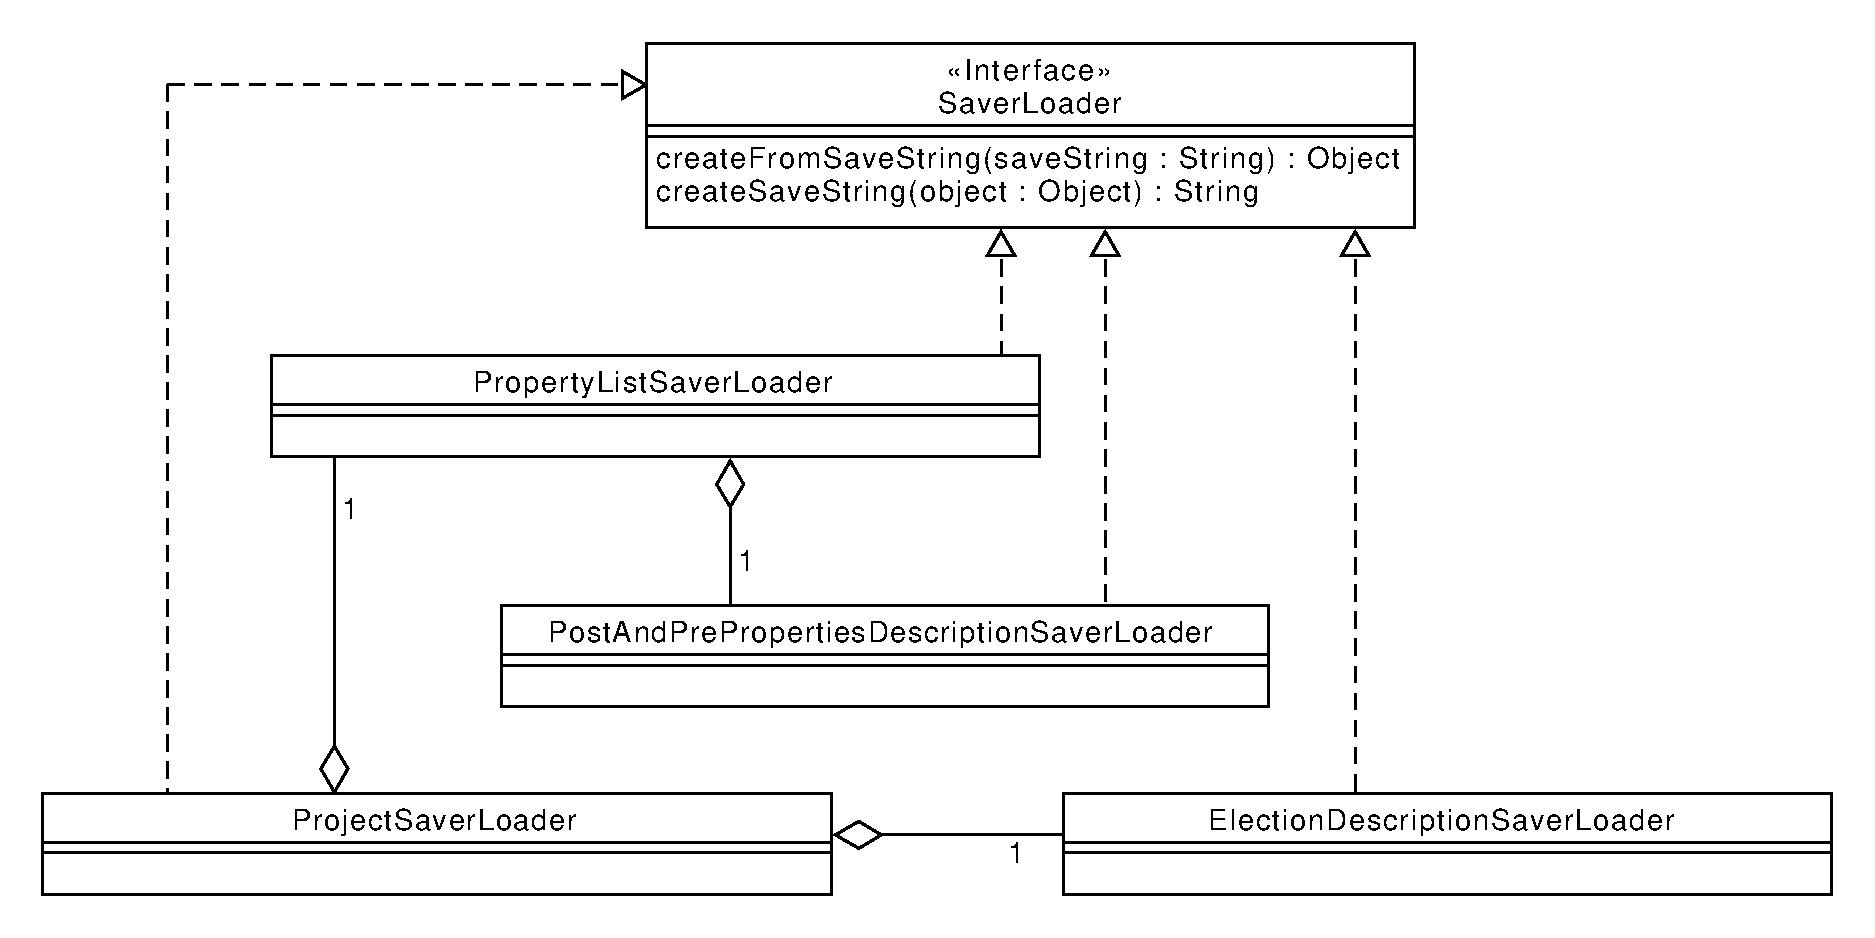
\includegraphics[scale=0.5]{SaverLoader.pdf}

\section{FileChooser}
Diese Klasse kümmert sich um das Laden und Speichern der speicherbaren Datentypen.
\newline
(Diagramm folgt)
\newline

\section{DataTypes}
Die als Datei abspeicherbaren Datentypen implementieren nun alle das Interface \\ \verb!ChangeNameInterface!, das es dem \verb!FileChooser! ermöglicht das name-Attribut dieser Klassen polymorph zu verändern.\\
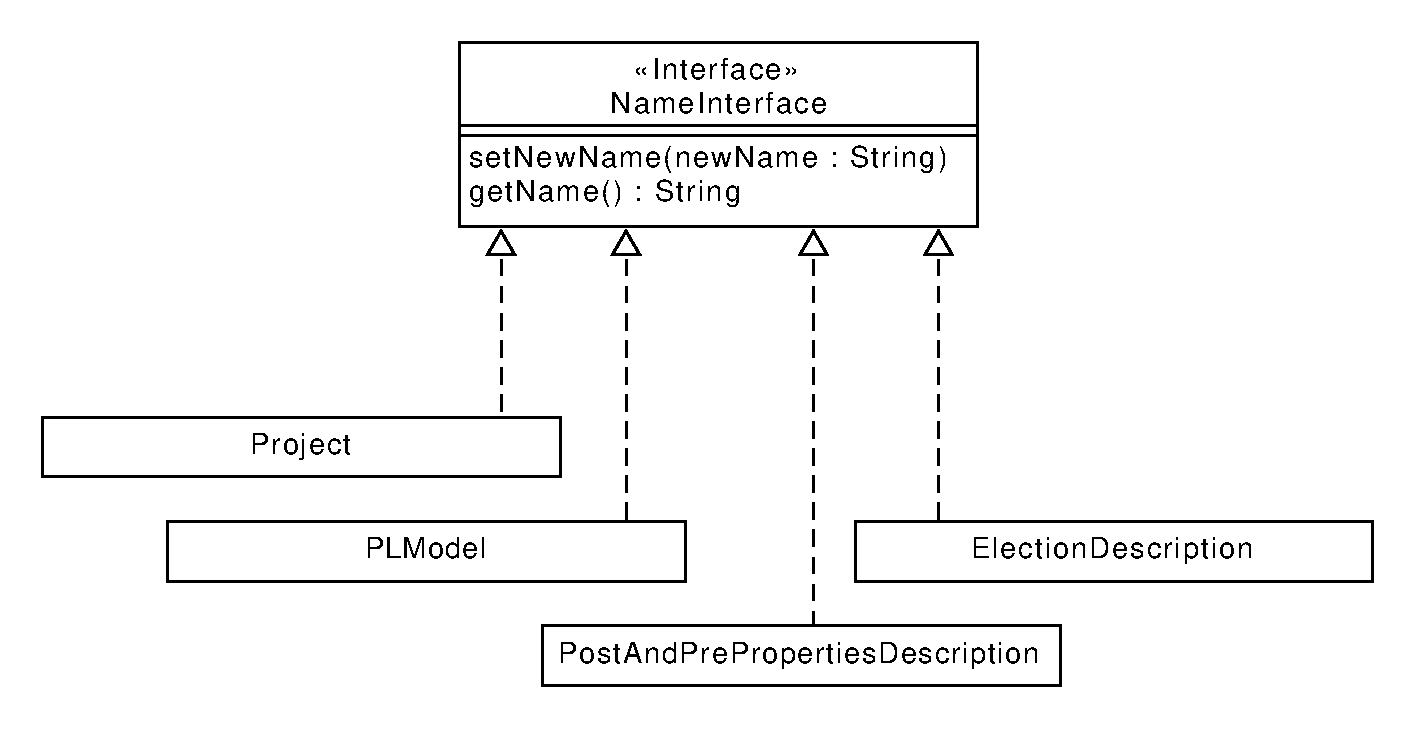
\includegraphics[scale=0.5]{NameInterface.pdf}


\section{Codearea}
\subsection{JTextPaneToolbox}
Klasse \verb!JTextPaneToolbox! wurde hinzugefügt. Diese enthält einige statische Methoden, welche oft benötigte, aber nicht zusammengehörige Funktionalität für \verb!JTextPane! liefern. Dazu gehört unter anderem das Umwandeln absoluter Positionen in Zeilennummern.\\
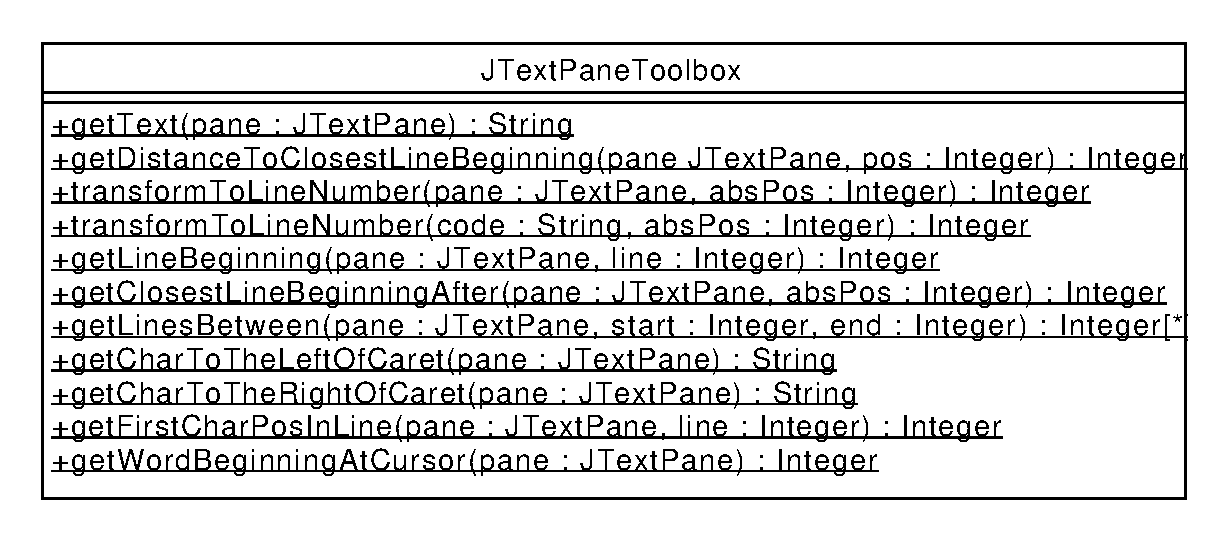
\includegraphics[scale=0.5]{JTextPaneToolbox.pdf}\\
\subsection{Errordisplayer}
\verb!Errordisplayer! ist nun abstrakt. Von den erbenden Klassen müssen Fehlermeldungen generiert werden.\\
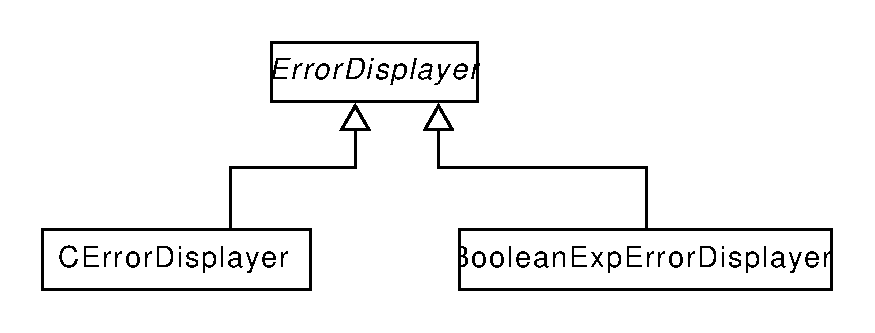
\includegraphics[scale=0.5]{Errordisplayer_update.pdf}\\
\subsection{SaveTextBeforeRemove}
DieKlasse \verb!SaveTextBeforeRemove! wurde hinzugefügt. Diese speichert den Text einer \verb!JTextPane!, sobald Text daraus entfernt wird. Dies ist nötig, da das \verb!RemovedUpdate! des Styleddocuments keinen Zugriff auf den entfernten Text gewährt. Dieser wird jedoch benötigt, um Aktionen rückgängig zu machen. Implementiert wird die Funktionalität durch hören auf Keyevents.\\
\subsection{TextLineNumber}
Klasse \verb!TextLineNumber! wurde hinzugefügt, welche die Zeilennummer anzeigt. Diese Klasse wurde direkt aus \\https://tips4java.wordpress.com/2009/05/23/text-component-line-number/ übernommen.\\
\subsection{SquigglePainter}
Klasse \verb!SquigglePainter! wurde hinzugefügt. Diese unterstreicht Text in der \verb!JTextPane! gezackt. Dies wird verwendet, um Fehler im Code anzuzeigen. Übernommen von 
https://tips4java.wordpress.com/2008/10/28/rectangle-painter/\\
\subsection{JTextPaneToolbox}

\subsection{Tabinserter}
\verb!Tabinserter! wurde hinzugefügt. Dieser fügt Tabs in Form von Leerzeichen ein.\\
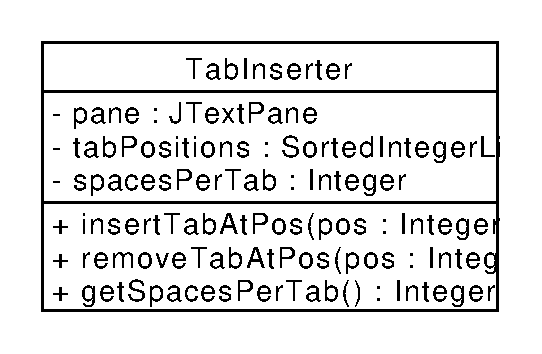
\includegraphics[scale=0.5]{TabInserter.pdf}\\
\subsection{LineBeginningTabsHandler}
Interface \verb!LineBeginningTabsHandler! und Implementierung \verb!CurlyBracesLineBeginningTabHandler! wurden hinzugefügt. \verb!LineBeginningTabsHandler! berechnet die benötigte Anzahl Tabs zu Beginn einer gegebenen Zeile. \verb!CurlyBracesLineBeginningTabHandler! errechnet dies anhand der Anzahl geöffneter curly-Braces in vorangehenden Zeilen minus die Anzahl schließender curly-Braces am Ende der gegebenen Zeile\\
\subsection{UserActions}
Es gibt nun spezielle \verb!UserActions! für Kopieren, Ausschneiden und Einfügen. Dies ist nötig um sicherzustellen, dass nicht editierbare Zeilen nicht durch diese Aktionen verändert werden.\\
\subsection{NewlineInserter}
\verb!NewlineInserter! ist nun ein eigenes Paket. \verb!BetweenCurlyBracesNewlineInserter! verwendet nun \verb!StandardNewlineInserter!.\\
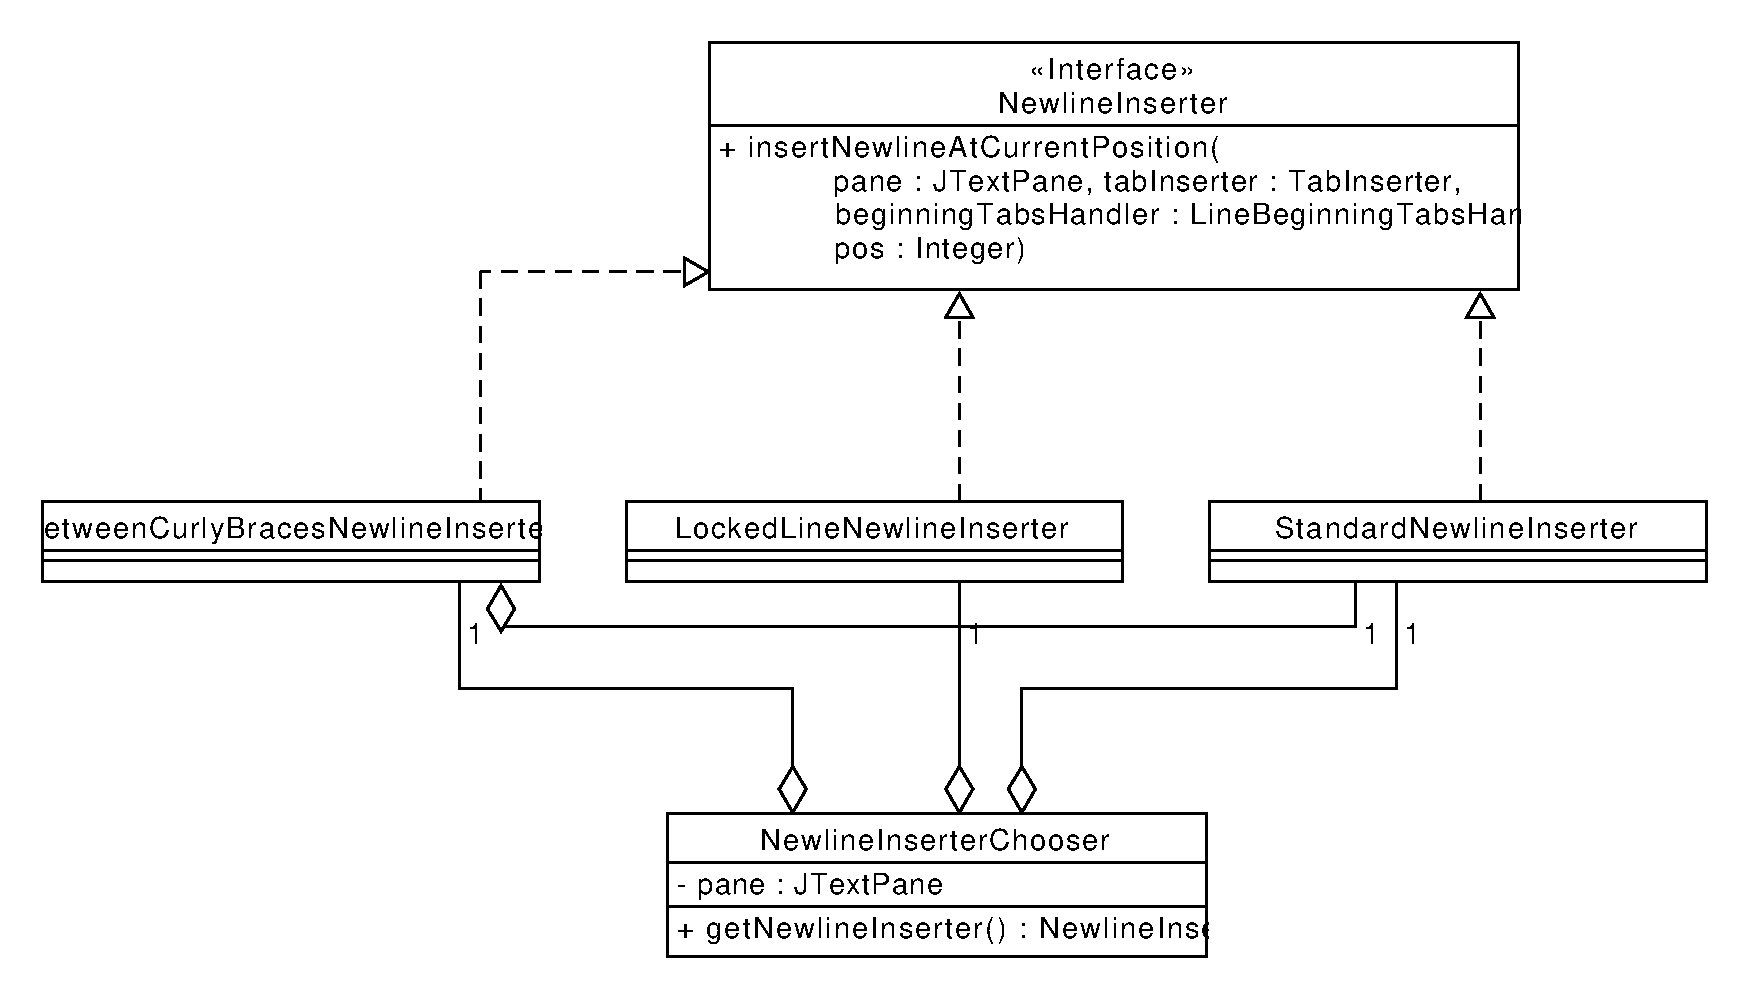
\includegraphics[scale=0.5]{insertnewline_update.pdf}


\subsection{UserInsertToCode}
Hinzu kommen folgende Funktionen:
\begin{itemize}
\item insertTab fügt an der Momentanen Position ein Tab ein
\item insertChar Fügt das gegebene Zeichen an der momentanen Position ein
\item getFirstLockedLine gibt die erste nicht editierbare Zeilennummer
\item moveToEndOfCurrentLine Bewegt den Caret ans Ende der momentanen Zeile
\item moveToStartOfCurrentLine Bewegt den Caret an den Start der momentanen Zeile
\item removeToTheRight Entfernt das Zeichen rechts vom Caret
\item removeToTheLeft Entfernt das Zeichen links vom Caret
\end{itemize}

Entfernt wurden:
\begin{itemize}
\item msgLockedLinesListeners: wird nun von \verb!LockedLineHandler! übernommen
\end{itemize}

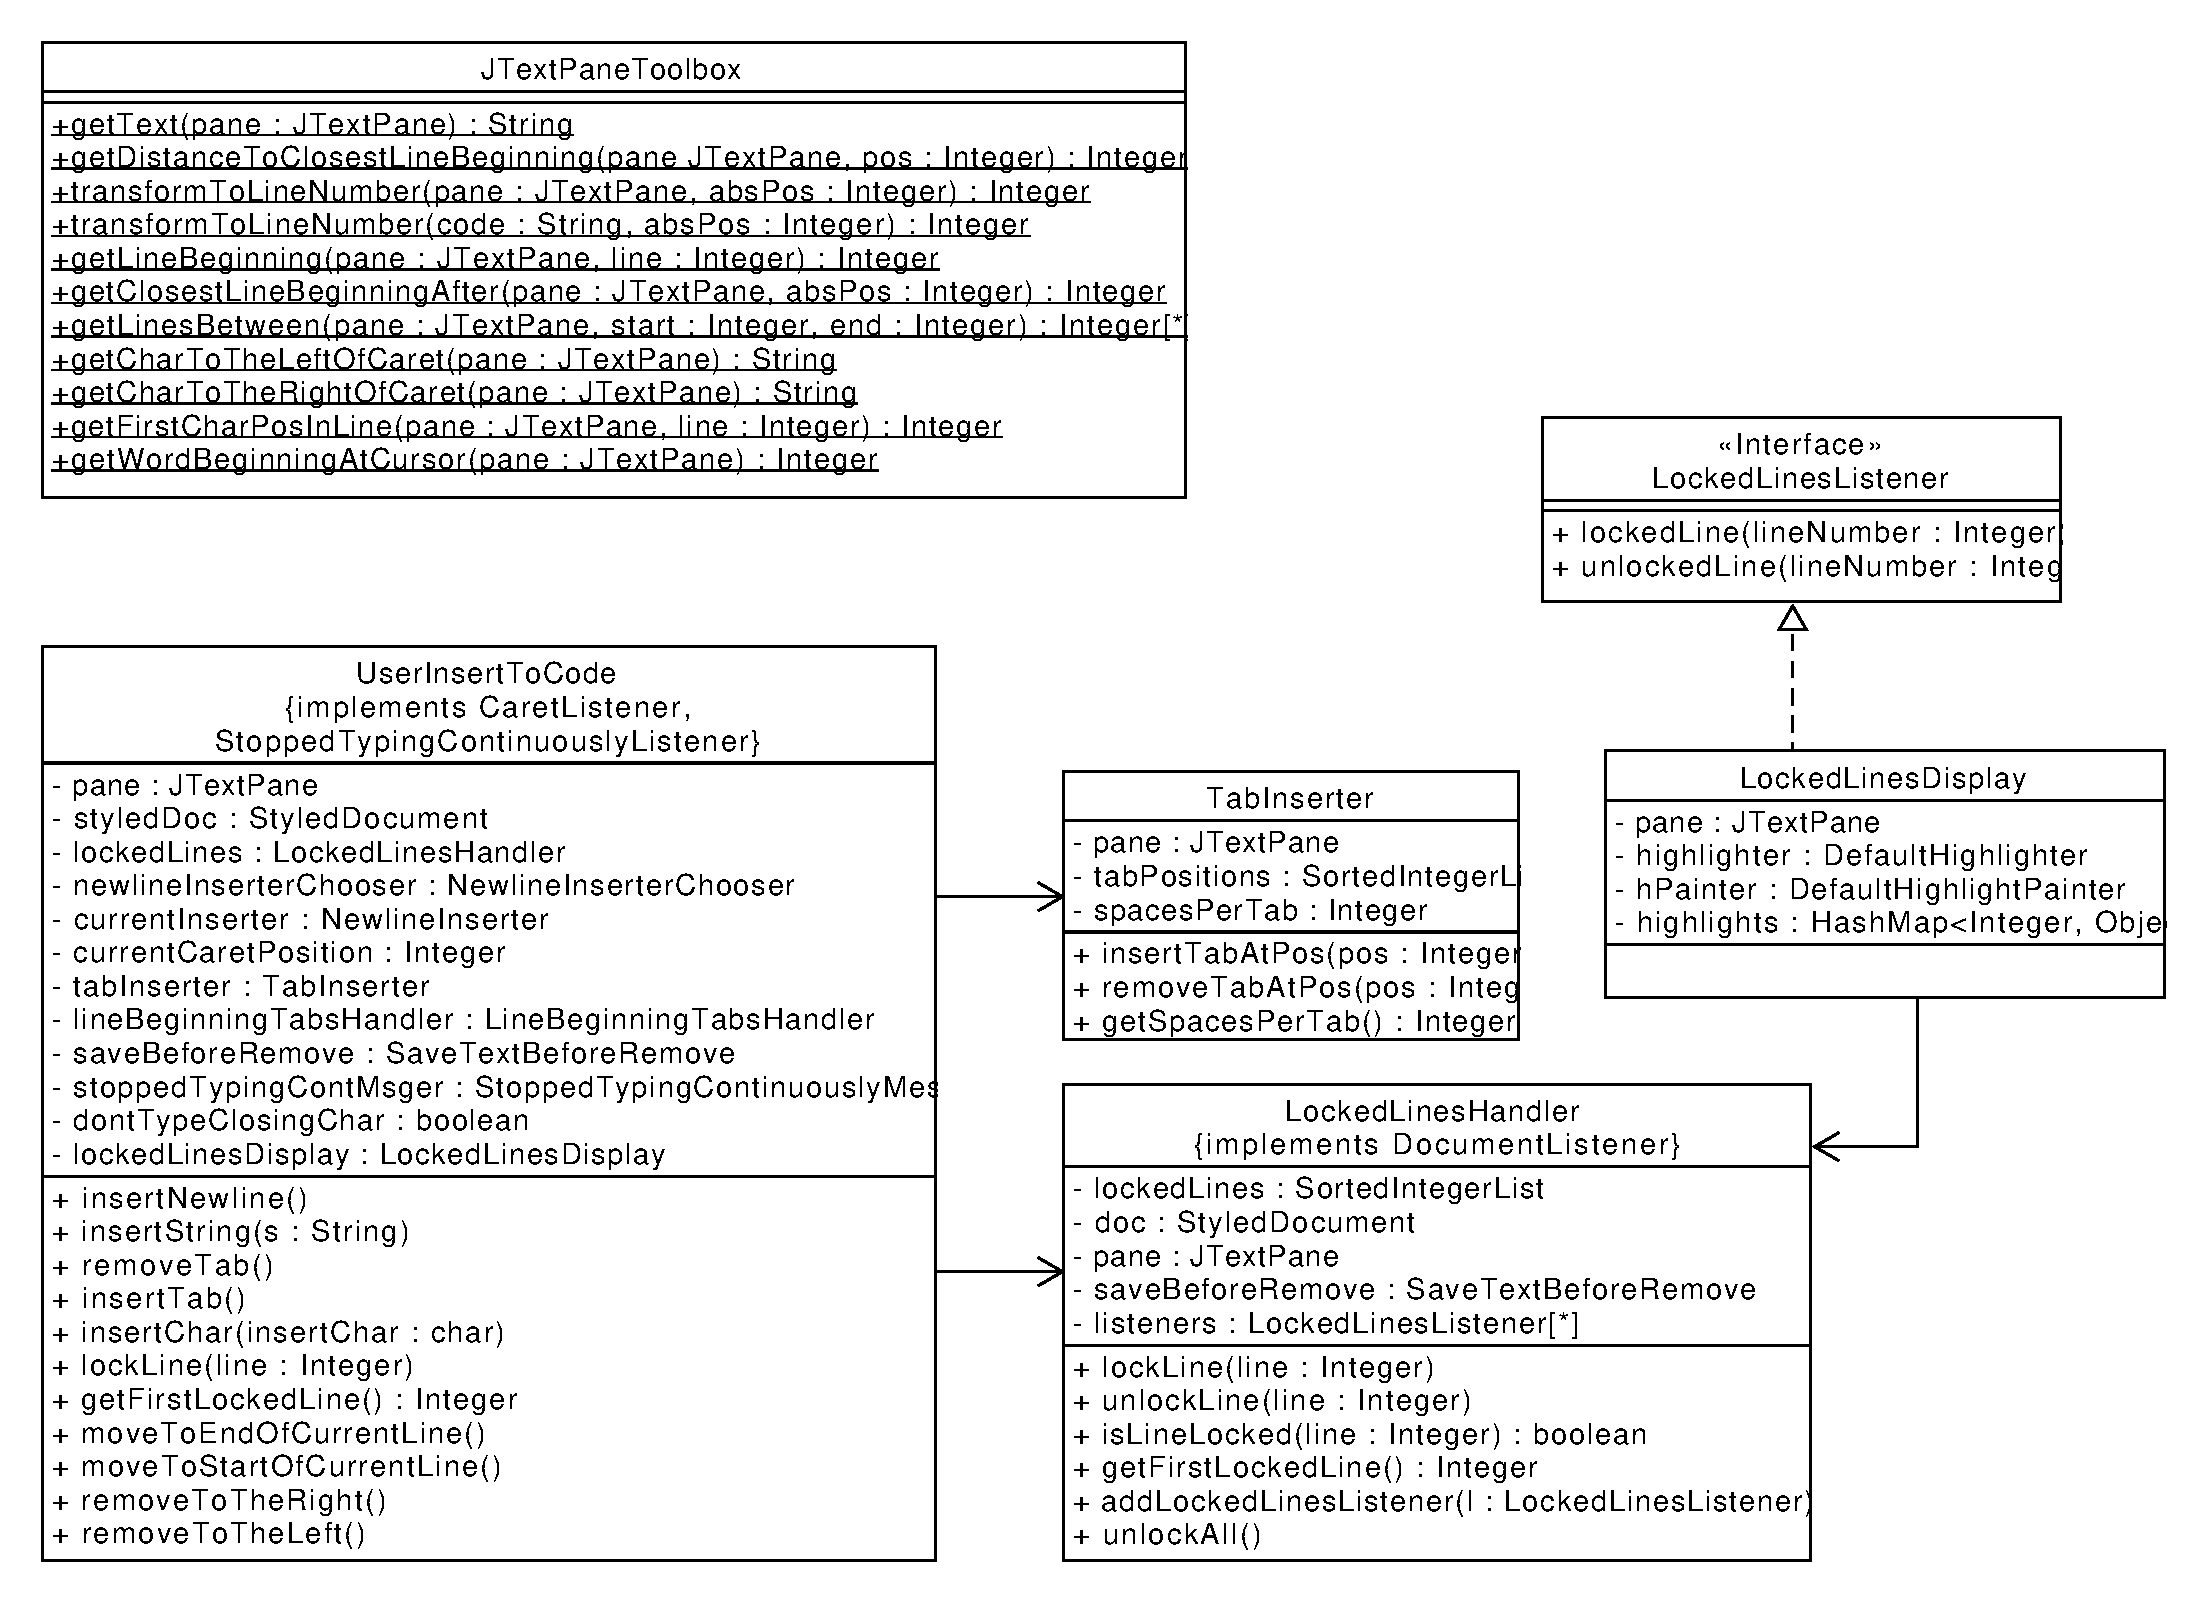
\includegraphics[scale=0.45]{inputtocode_update.pdf}

\section{BooleanExpEditor}
Der \verb!BooleanExpEditor! besitzt jetzt eine Referenz auf die \verb!CElectonDescriptionEditor!-Instanz, da dies zur Fehlerfindung durch den \verb!BooleanExpEditorVariableErrorFinder! nötig ist.
\newline
Er bekommt vom Builder nun eine Referenz auf die \verb!PropertyList!-Instanz, da so neu erstellte Eigenschaften in der Liste gespeichert werden können.
\newline
(Diagramm folgt)
\newline

\section{CElectionDescriptionEditor}

- Die \verb!ChangeElectionType! \verb!UserAction! und der entsprechende Menüpunkt "Wahlart ändern" wurden entfernt. \\
- Das neue Paket \verb!ElectionTemplates! kam hinzu. Dieses enthält folgende Klassen:\\
\begin{itemize}
\item \verb!ElectionTemplateHandler!: Gibt alle Election Input und Output Datentypen und deren ids aus.
\item \verb!ElectionTemplateChooser!: Zeigt dem Benutzer einen Dialog, welcher es ermöglicht Input und Result eines neuen Wahlverfahrens zu wählen.
\end{itemize}
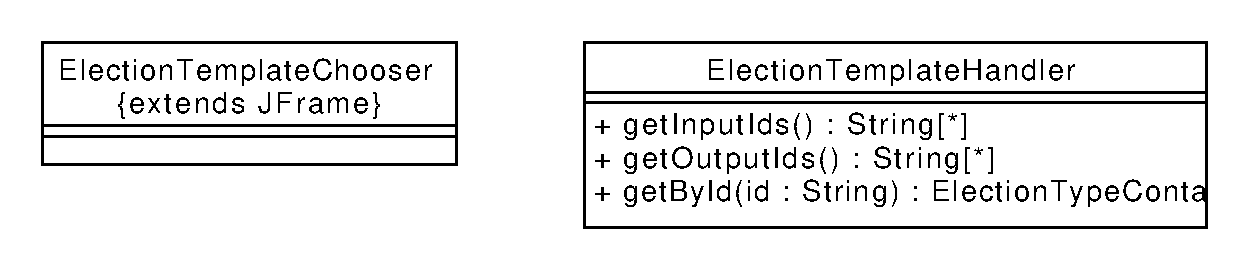
\includegraphics[scale=0.5]{ElectionTemplates.pdf}\\

\subsection{ErrorHandling}
Die C-Fehlerfindung findet nun ausschließlich über Aufruf eines externen Compilers statt. Dieser Aufruf geschieht und das Parsen seiner Rückgabe findet in den Klassen \verb!DeepErrorChecker!, \verb!LinuxErrorChecker!, \verb!WindowsErrorChecker! und \verb!SystemSpecificErrorChecker! statt.
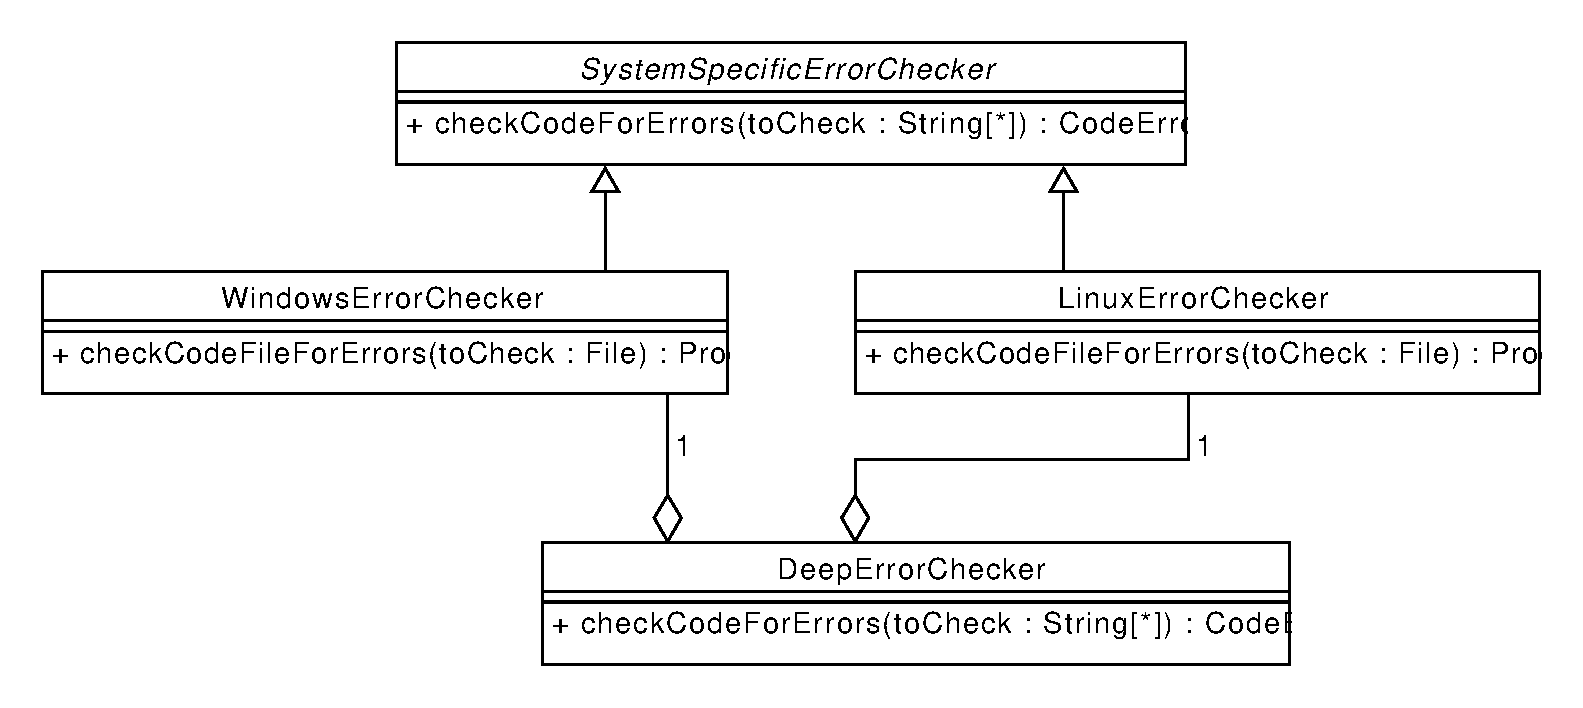
\includegraphics[scale=0.5]{CErrorChecking.pdf}

\section{PropertyChecker}
Beim \verb!PropertyChecker! hat sich folgendes im Vergleich zum Entwurf
verändert:

\begin{itemize}
\item Die Klasse \verb!CBMCResult! besitzt nun die Methode
``createFailureExample'' samt zugehöriger Untermethoden, welche zur Erstellung des Failurexamples
  genutzt werden. Deshalb besitzt die Klasse \verb!Checker! diese Fähigkeit nicht mehr.

\item Es wurden drei neue Klassen
\footnote{CBMCResultWrapper/long/singleArray/multiArray} erstellt, welche
beim Parsen der Ergebnisse von CBMC mithelfen. Sie werden während des Parsens der Rückgabe von CBMC verwendet, um die Teilergebnisse in Listen zu speichern und sie am Ende als Array ausgeben zu können. Dies wurde auf diese Weise implementiert, da am
Anfang des Parsens nicht bekannt sein kann, wie groß die Datentypen bei der
Rückgabe werden würden und es die eigentliche Methode ``createFailureExample''
deutlich verkürzen konnte.

\item Die Klasse \verb!CheckerFactory! besitzt nun zwei neue Methoden: \newline
``getNewInstance(\ldots)'' wird dazu verwendet eine neue Instanz einer
\verb!CheckerFactory! zu erstellen, damit die \verb!CheckerFactoryFactory! neue \verb!CheckerFactorys!
erstellen kann. \newline Außerdem gibt es nun die Methode ``getMatchingResult(int
amount)'', welche die gewünschte Anzahl an checkerspezifischen \verb!Result! Objekten
zurückgibt, sodass die \verb!CheckerFactoryFactory! von diesen dann auf Wunsch so viele
wie nötig erstellen kann.

\end{itemize}


\section{PropertyList}

Das Paket \verb!PropertyList! hat sich im Unterpaket \verb!Controller! geändert. Durch die Anbindung an die \verb!highlevel!-Interfaces wurde es nötig, dass das Model der \verb!PropertyList! kein Einzelstück mehr ist. Der Controller benötigt deshalb eine eigene Referenz auf das Model, weil er nicht auf die einzelne Instanz zugreifen kann. Eine zentrale Controllerklasse übernimmt nun die Steuerung, anstatt wie vorgesehen einzelne Klassen.

Die Methoden für Controller und Model wurden außerdem in eigenen Interfaces beschrieben, sodass ein schneller Überblick über die Methoden gegeben ist.

\subsection{Subpackage Model}
Die Klasse \verb!PropertyList! wurde zu \verb!PLModel! umbenannt. Sie hat keine Anbindung nach außerhalb des Pakets mehr. Das Interface \verb!PostAndPrePropertiesDescriptionSource! wird nun vom Controller implementiert.

Die Klasse \verb!PropertyItem! hält nun Daten zum Ergebnis der Analyse (zusätzlich zu \verb!PropertiesDescription! und Teststatus).

Das Interface \verb!PLModelInterface! beschreibt alle Manipulationen der Eigenschaftenliste.

\subsection{Subpackage Controller}
Die zentrale Klasse des Controllers heißt \verb!PropertyList! und implementiert alle nötigen Interfaces nach außen. Das sind:
\begin{itemize}
	\item \verb!ResultPresenter! (im Entwurf nur vom View implementiert)
	\item \verb!PostAndPrePropertiesDescriptionSource! (eigentlich im Entwurf im Model implementiert)
	\item \verb!Runnable! (Klasse startet den View)
	\item \verb!DisplaysStringsToUser! (zur Entgegennahme der Strings für den View)
	\item \verb!PLControllerInterface! (alle möglichen Befehle für die \verb!PropertyList!)
\end{itemize}
Die \verb!Action!- und \verb!ChangeListener! wurden aus dem Controller rausgezogen und direkt im View implementiert.

Die Klassen, die \verb!ListChangeCommand! erweiterten (\verb!ChangeDescription!, \verb!ChangeDescriptionName!, \verb!AddStandardDescription!, \verb!AddNewDescription!, \verb!ChangeTestedStatus!, \verb!Redo!, \verb!Undo!), sind nur noch Methoden im Interface des Controllers (void changeName(PropertyItem prop, String newName); usw.). Das geschah, weil sie so kleine Änderungen an der \verb!PropertyList! bedeuten, dass sie nicht rückgängig gemacht werden müssen. Stattdessen kann der Nutzer neu erstellte Eigenschaften mit dem Klick auf den entsprechenden Button wieder löschen. Lediglich \verb!DeleteDescriptionAction! ist den Undo wert und wurde deshalb in einer eigenen Klasse gekapselt.

Der \verb!SaveBeforeChangeHandler! war im Entwurf noch nicht beschrieben.

\subsection{Subpackage View}
Die Elemente des View sind großteils gleich geblieben. Sie wurden allerdings nicht mit einem GUI-Builder erstellt, weil dann nicht dynamisch Komponenten hinzugefügt werden könnten (Formulare mit fester Anzahl von Komponenten).

Im Entwurf war angedacht, dass das Model die View direkt von Änderungen benachrichtigt. Nun wird das Beobachtermuster benutzt, um dem View Änderungen im Model mitzuteilen. In diesem Falle wird die Liste der Eigenschaften (ArrayList<ListItem>) neu aufgebaut.

Neu hinzugekommen ist die Klasse \verb!ResultPresenterWindow!, die die Swing-Klasse \verb!JFrame! erweitert. Dadurch war es nicht möglich, sie als Kinder des Hauptfensters zu deklarieren. Aber durch die Entscheidung gegen eine \verb!JTextPane! konnte das Layout aus dem Pflichtenheft besser dargestellt werden.

\section{Package Parametereditor}

Das Paket \verb!parametereditor! umfasst die Klassen, die das Hauptfenster von BEAST (das Parametereditorfenster) aufbauen und die dortigen Eingaben des Nutzers verarbeiten. In diesem Fenster können Parameter für die Analyse des Wahlverfahrens (Anzahl von Wählern, Kandidaten und Stimmen, sowie maximale Anzahl von Prozessen und maximale Dauer der Analyse) angegeben werden. Außerdem können hier benutzerdefinierte Argumente für CBMC angegeben und die Analyse gestartet und gestoppt werden.

\subsection{Class ParameterEditor}
Die Klasse \verb!ParameterEditor! implementiert jetzt nicht mehr \verb!BEASTCommunicator! aus \verb!highlevel!. Damit wird \verb!ParameterEditor! klar von der Kommunikation zwischen den einzelnen Teilen von BEAST getrennt. \\

\subsection{UserActions}
Es wurden neue \verb!UserActions! hinzugefügt:
\begin{itemize}
\item \verb!NewProjectUserAction!, um neben Laden und Speichern auch das Erstellen eines neuen Projekts zu ermöglichen.
\item \verb!OptionsUserAction!, um es dem Nutzer zu ermöglichen, Einstellungen wie etwa die Sprache zu ändern.
\item \verb!ShowHideBooleanExpEditor!, \verb!ShowHideCElectionEditor! und \verb!ShowHidePropertyList!, um die anderen GUI-Fenster vom Parametereditor aus öffnen und schließen zu können.
\end{itemize}

\subsection{Handlers}
Es wurden neue Handler hinzugefügt:
\begin{itemize}
\item \verb!ArgumentHandler!, um die benutzerdefinierten Argumente für CBMC zu verarbeiten.
\item \verb!SaveBeforeChangeHandler!, um sicherzustellen, dass der Nutzer nicht versehentlich durch Laden oder Erzeugen eines neuen Projekts ein ungespeichertes Projekt verwirft.
\end{itemize}

\subsection{AboutWindow}
Es wurde die Klasse \verb!AboutWindow! hinzugefügt, die dem Nutzer das Akronym BEAST erklären und die aktuelle Versionsnummer sowie das Build-Datum anzeigt.

\section{Toolbox}
Folgende Klassen kamen hinzu:\\
- \verb!SortedIntegerList!: Eine einfache Wrapperklasse, welche eine stets sortierte Liste von Integern enthält. Diese wird verwendet von \verb!LockedLinesHandler! und \verb!TabInserter!.\\
- \verb!RepaintThread!: Implementiert \verb!Runnable!. Bekommt einen \verb!JFrame! für welchen er 60 Mal pro Sekunde die repaint-Funktion aufruft. Dies ist benötigt, da die Frames auf Windows sonst nicht korrekt rendern, falls zuvor ein anderes Fenster vor ihnen war.\\
- \verb!CCodeHelper!: Diese Klasse enthält Funktionalität um aus den internen Datentypen C Code zu erstellen. Sie wird sowohl von der Codegenerierung als auch dem C-Editor verwendet. \\
- \verb!ActionIdAndListener!: Eine einfache Wrapper-Klasse welche Zugriff auf einen \verb!ActionListener! und die dazugehörige String-Id bietet.\\
- \verb!Tuple!: Eine Klasse, welche zwei verschiedene Typen hält.

\chapter{Zeitablauf Implementierungsphase}

\section{Geplanter Ablauf}

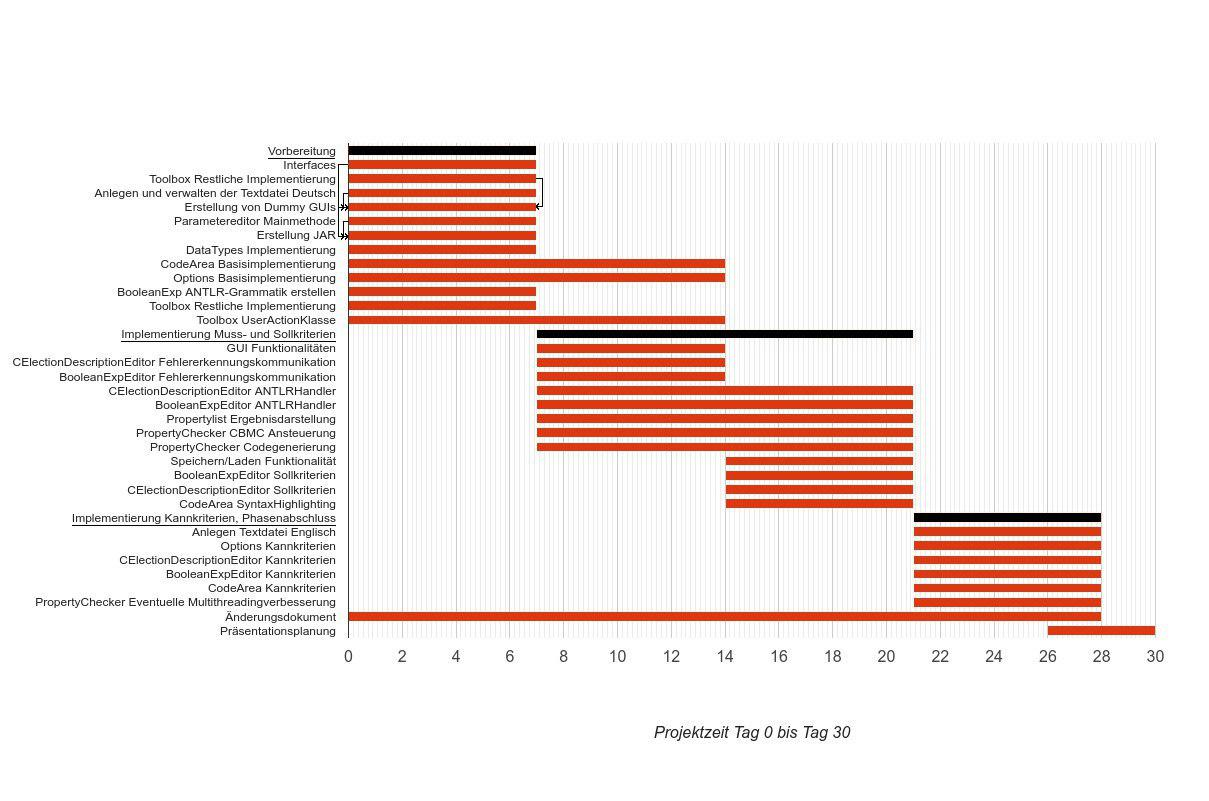
\includegraphics[width=1.3\textwidth] {originalPlanung.jpg}

\section{Eigentlicher Ablauf}
Der ursprüngliche Plan wurde hauptsächlich eingehalten. Ein paar Komplikationen bei den Paketen \verb!highlevel!, \verb!parametereditor! und \verb!propertylist! verzögerten die Fertigstellung einiger Meilensteine.

(Genauere Beschreibung von Aufgabenumverteilung bzw. Ablaufänderung folgt)

(GANTT Diagramm von tatsächlichem Ablauf folgt)

\end{document}